\documentclass[11pt,a4paper]{article}
\usepackage[margin=2.2cm]{geometry}
\usepackage[T1]{fontenc}
\usepackage[utf8]{inputenc}
\usepackage{booktabs}
\usepackage{graphicx}
\usepackage{float}
\usepackage{listings}
\usepackage{xcolor}
\usepackage{enumitem}
\usepackage{fancyhdr}
\usepackage[colorlinks=true,linkcolor=blue,urlcolor=blue]{hyperref}
\usepackage{caption}
\usepackage{amsmath}

\definecolor{codebg}{RGB}{247,247,247}
\definecolor{notebg}{RGB}{238,243,251}
\lstset{
  language=C++,
  basicstyle=\ttfamily\footnotesize,
  backgroundcolor=\color{codebg},
  frame=single, framerule=0.4pt, rulecolor=\color{gray!60},
  breaklines=true, breakatwhitespace=true,
  showstringspaces=false,
  keywordstyle=\color{blue!70!black}\bfseries,
  commentstyle=\color{green!40!black}\itshape,
  stringstyle=\color{red!60!black},
  numbers=left, numberstyle=\tiny\color{gray}, numbersep=6pt,
  xleftmargin=1.2em, framexleftmargin=1.2em,
  tabsize=2
}
\lstdefinestyle{out}{language={}, basicstyle=\ttfamily\small, numbers=none, xleftmargin=0pt, framexleftmargin=0pt, backgroundcolor=\color{notebg}}
\lstdefinestyle{pseudo}{language={}, basicstyle=\ttfamily\small, numbers=none, xleftmargin=0pt, framexleftmargin=0pt, frame=single, backgroundcolor=\color{notebg}, breaklines=true}

\newcommand{\notebox}[1]{\par\medskip\noindent\fbox{\parbox{\dimexpr\linewidth-2\fboxsep-2\fboxrule}{\small #1}}\par\medskip}
\newcommand{\lstout}[2]{\lstinputlisting[style=out,caption={#2},label={#1}]{#1}}

\pagestyle{fancy}
\fancyhf{}
\lhead{DSA01 -- Assignment 5 (CO5)}
\rhead{H Saravana \;|\; 192511397}
\cfoot{\thepage}

\title{\textbf{Assignment 5 -- CO5}\\[4pt]Reliable Software with Runtime Polymorphism and Exceptions\\[6pt]\large Hospital Billing and Insurance Claims}
\author{}
\date{}

\begin{document}

\begin{titlepage}
\centering
\vspace*{1cm}
{\Huge\bfseries Assignment 5 -- CO5}\\[10pt]
{\Large Reliable Software with Runtime Polymorphism and Exceptions}\\[30pt]
{\large Course: DSA01 \qquad Nature: Individual \qquad Total Marks: 50}\\[40pt]
\begin{tabular}{@{}ll@{}}
\toprule
\textbf{Student name} & H SARAVANA \\
\textbf{Register number} & 192511397 \\
\midrule
\textbf{Compiler} & g++ 13.3.0 (Ubuntu 13.3.0-6ubuntu2\~24.04.1) \\
\textbf{Compile command} & \texttt{g++ -std=c++17 -Wall -Wextra} \\
\textbf{Sanitizers} & \texttt{-fsanitize=address} (and \texttt{undefined} where stated) \\
\textbf{Timing build} & \texttt{g++ -std=c++17 -O2 -Wall -Wextra} \\
\midrule
\textbf{GitHub repository} & \texttt{https://github.com/<your-username>/DSA01-192511397-Assignment5} \\
\bottomrule
\end{tabular}
\vfill
{\small The GitHub link above must be replaced with the student's own repository URL before submission.}
\end{titlepage}

\tableofcontents
\newpage

%=============================================================
\section{Summary of Work}
%=============================================================
Every task in the assignment has an implementation or a design artefact, and every program was compiled and run with the commands above. The table gives the evidence location for each deliverable. The repository folder names match the task numbers.

\begin{table}[H]
\centering
\small
\begin{tabular}{@{}llp{8.2cm}@{}}
\toprule
\textbf{Task} & \textbf{Part} & \textbf{Evidence (repository)} \\
\midrule
A1 & Polymorphic hierarchy & UML (Fig.~\ref{fig:uml}), pseudocode in Sec.~\ref{sec:a1} \\
A2 & Runtime binding & Vtable figure (Fig.~\ref{fig:vtable}), \texttt{Task01\_Binding\_VirtualDtor/} \\
A3 & Payer abstraction & Fig.~\ref{fig:payer}, \texttt{Task06\_Extension\_Final/billing.hpp} \\
A4 & Exception strategy & Fig.~\ref{fig:exc}, \texttt{Task04\_ErrorHandling/error\_tests.cpp} \\
A5 & Recovery and rethrow & \texttt{Task02\_RAII\_Unwinding/} \\
B1 & Implementation and binding proof & \texttt{Task03\_Billing\_CompleteCode/}, \texttt{Task06\_Extension\_Final/main.cpp} \\
B2 & Error conditions & \texttt{Task04\_ErrorHandling/} \\
B3 & Performance measurement & \texttt{Task05\_Performance/bench.cpp} \\
B4 & Extension and decision & \texttt{Task06\_Extension\_Final/extension.hpp} \\
\bottomrule
\end{tabular}
\end{table}

\notebox{\textbf{Note on predictions and submission.} The assignment requires each predicted output to be written before the program is run. The predictions in this report were derived from the C++ rules before the programs were executed, but they must be written out again by the student before running each program for credit. Pseudocode follows a consistent structured notation with numbered steps; the SIMATS standard document was not included with the upload and should be checked against it. The GitHub repository must contain a commit history with at least one commit per task.}

%=============================================================
\part*{Part A -- Design}
\addcontentsline{toc}{part}{Part A -- Design}
%=============================================================

\section{Task A1 -- Polymorphic Bill Hierarchy}\label{sec:a1}

\subsection*{A1.1 Common interface}
Every bill must answer three questions and carries one piece of shared data:
\begin{itemize}[nosep]
\item \textbf{total()}: the amount payable (pure virtual; each bill kind has its own rule).
\item \textbf{type()}: a short code (\texttt{OP}, \texttt{IP}, \texttt{DC}) used for reports (pure virtual).
\item \textbf{print()}: a fixed format built from the two above (non-virtual, so every bill prints the same way).
\item \textbf{Shared data}: the patient name.
\end{itemize}

\subsection*{A1.2 Hierarchy and UML}
An abstract base class \texttt{Bill} declares \texttt{total()} and \texttt{type()} as pure virtual and has a virtual destructor. Each concrete class overrides both functions. Figure~\ref{fig:uml} is the UML class diagram.

\begin{figure}[H]
\centering
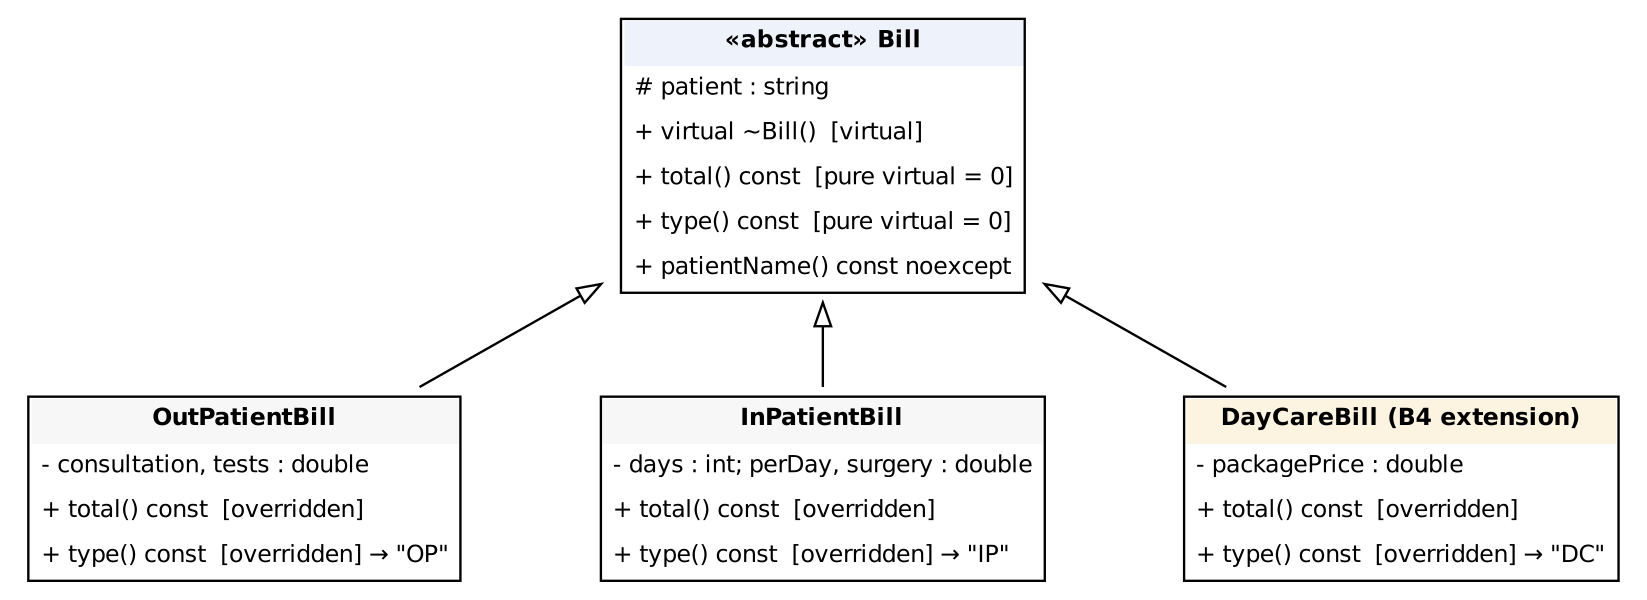
\includegraphics[width=0.95\linewidth]{uml_bill.png}
\caption{UML class diagram of the bill hierarchy. Stereotype and modifiers mark which members are virtual, pure virtual, or overridden.}\label{fig:uml}
\end{figure}

\begin{table}[H]
\centering
\small
\begin{tabular}{@{}lccc@{}}
\toprule
\textbf{Member} & \textbf{Bill} & \textbf{OutPatientBill} & \textbf{InPatientBill} \\
\midrule
\texttt{\~{}Bill()} (destructor) & virtual & overridden (implicit) & overridden (implicit) \\
\texttt{total() const} & pure virtual & overridden & overridden \\
\texttt{type() const} & pure virtual & overridden (``OP'') & overridden (``IP'') \\
\texttt{print() const} & non-virtual & inherited & inherited \\
\bottomrule
\end{tabular}
\caption{Marking of virtual, pure virtual and overridden functions.}
\end{table}

\subsection*{A1.3 Processing all bills together}
The day's total is computed over an array of base-class pointers. The loop contains one virtual call per bill, and the correct \texttt{total()} is chosen at run time.

\begin{lstlisting}[style=pseudo,caption={Pseudocode: day total over base-class pointers}]
ALGORITHM DayTotal(bills, n)
  INPUT : bills -- array of n pointers of type Bill*
  OUTPUT: sum   -- the day's total
  BEGIN
    sum <- 0
    FOR i <- 0 TO n - 1 DO
      sum <- sum + bills[i]->total()     // virtual call, bound at run time
    END FOR
    RETURN sum
  END
\end{lstlisting}

\subsection*{Alternative concept: one struct with a type field and a switch}
Instead of a class hierarchy, one \texttt{Bill} record holds a \texttt{kind} field and \texttt{total()} contains a \texttt{switch}. Time to total $n$ bills is $O(n)$ in both designs. The switch record is a 24-byte value stored inline in an array. The virtual objects are 24 bytes (\texttt{VOP}) or 32 bytes (\texttt{VIP}) plus a heap allocation header and an 8-byte \texttt{unique\_ptr} per element, so the virtual design uses more space per bill (measured in B3). The more important difference is the cost of extension. A new bill type forces edits in every switch statement across the code base, which breaks the open--closed principle. A new derived class needs no change to existing classes. The experiments in B3 measure the constant factors.

%-------------------------------------------------------------
\section{Task A2 -- Understanding Runtime Binding}
%-------------------------------------------------------------
\subsection*{A2.1 Early and late binding}
Early (compile-time) binding is used for non-virtual functions: the compiler picks the function from the static type of the pointer and emits a direct call. Late (run-time) binding is used for virtual functions: with \texttt{Bill* b}, the compiler cannot know the object's dynamic type, so it emits an indirect call through the object's vtable. The call \texttt{b->total()} is therefore resolved when the program runs, after the object exists.

\subsection*{A2.2 Virtual tables}
Each polymorphic class has one vtable (an array of function pointers), and each object has a hidden pointer, the vptr, to its class's vtable. Figure~\ref{fig:vtable} shows the three vtables of \texttt{Bill}, \texttt{OutPatientBill} and \texttt{InPatientBill}. Entry numbers are illustrative.

\begin{figure}[H]
\centering
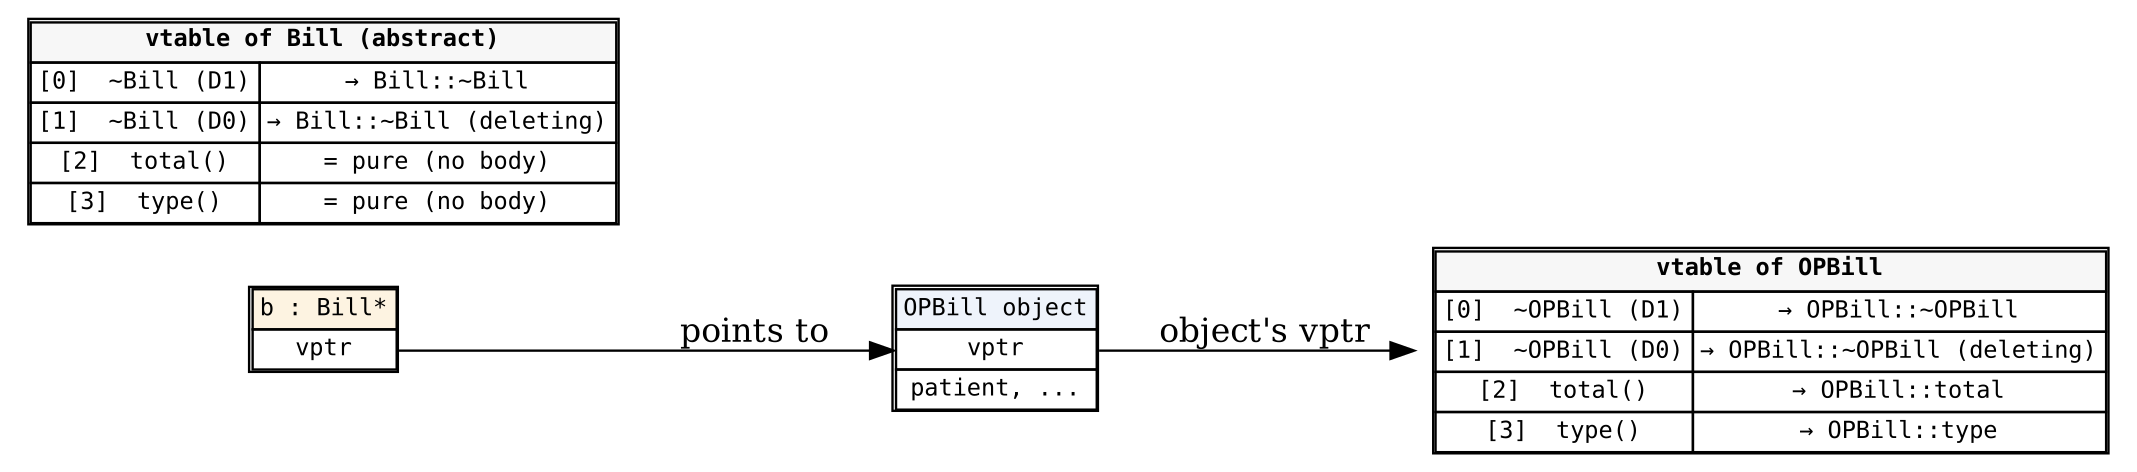
\includegraphics[width=0.9\linewidth]{vtable.png}
\caption{Vtable of \texttt{OPBill} and the abstract \texttt{Bill}. The pointer \texttt{b} reaches \texttt{OPBill::total} through the object's vptr and slot~2.}\label{fig:vtable}
\end{figure}

\noindent The call \texttt{b->total()} proceeds in three steps: (1) load the vptr from the object, (2) load the function pointer at the \texttt{total} slot of that vtable, (3) make an indirect call. Step 2 is the difference from a normal call. \textbf{For InPatientBill}, the same steps reach \texttt{InPatientBill::total} from its own vtable, which has a different function at slot~2.

The complete vtable list is:
\begin{itemize}[nosep]
\item \texttt{Bill}: destructor entries (pointing to \texttt{Bill::\~{}Bill}), \texttt{total} and \texttt{type} are pure (no body, so the entry is a null marker).
\item \texttt{OutPatientBill}: destructor entries pointing to \texttt{OutPatientBill::\~{}OutPatientBill}, \texttt{total} $\to$ \texttt{OutPatientBill::total}, \texttt{type} $\to$ \texttt{OutPatientBill::type}.
\item \texttt{InPatientBill}: the same layout, with \texttt{InPatientBill} functions in the total and type slots.
\end{itemize}

\subsection*{A2.3 Virtual destructors}
\texttt{delete b} with \texttt{Bill* b} calls the destructor through the pointer's static type. If \texttt{Bill}'s destructor is not virtual, only \texttt{Bill::\~{}Bill} runs. The derived destructor is skipped, so members of the derived class (for example a \texttt{std::vector} owning heap memory) are never released, and the memory is deallocated with the wrong size. The language makes this \emph{undefined behaviour}. A virtual destructor makes the call dispatch through the vtable, so the derived destructor runs first and the base destructor runs last.

\subsection*{Predict the output: program 1}
The program is given in the assignment (\texttt{Task01\_Binding\_VirtualDtor/predict\_a2.cpp}).

\begin{lstlisting}[caption={predict\_a2.cpp (as given)}]
#include <iostream>
struct Bill {
 virtual ~Bill() { std::cout << "~Bill "; }
 virtual double total() const = 0;
 void show() const { std::cout << total() << ' '; }
};
struct OPBill : Bill {
 ~OPBill() override { std::cout << "~OPBill "; }
 double total() const override { return 500; }
};
int main()
{
 Bill* b = new OPBill;
 b->show();
 delete b;
 std::cout << '\n';
}
\end{lstlisting}

\textbf{Predicted output (derived from the rules):} \texttt{500 \~{}OPBill \~{}Bill} followed by a newline.

\textbf{Actual output} (from \texttt{predict\_a2.out}):
\lstout{../Task01_Binding_VirtualDtor/predict_a2.out}{Actual output of predict\_a2}

\textbf{Explanation of the result.} \texttt{show()} is not virtual, but it calls \texttt{total()}, which is virtual. Inside \texttt{show()} the expression \texttt{total()} is \texttt{this->total()}, and \texttt{this} points to an \texttt{OPBill}. Its vptr therefore reaches \texttt{OPBill::total}, and the value 500 is printed. A non-virtual function can call a virtual one, and the dispatch still happens at run time. The destructor order matches the prediction: \texttt{OPBill}'s destructor runs first, then \texttt{Bill}'s.

\subsection*{Break test: non-virtual destructor, then ASan}
The \texttt{virtual} keyword is removed from \texttt{\~{}Bill}. The variant with \texttt{override} on \texttt{\~{}OPBill} fails to compile, because a derived destructor cannot override a non-virtual base destructor (see \texttt{compile\_error\_override.txt}). That variant was then modified so that \texttt{OPBill} owns a \texttt{std::vector}, which makes the skipped destructor observable.

\lstout{../Task01_Binding_VirtualDtor/nonvirtual_dtor.cpp}{Non-virtual destructor version (listing)}
\lstout{../Task01_Binding_VirtualDtor/nonvirtual_dtor.out}{Output of the non-virtual destructor version}

\textbf{Predicted output:} with \texttt{-fsanitize=address} the object is deleted as the wrong type. The derived destructor is skipped, so \texttt{\~{}OPBill} is never printed.

\textbf{Actual ASan result} (\texttt{nonvirtual\_dtor\_asan.out}):
\begin{lstlisting}[style=out]
==169==ERROR: AddressSanitizer: new-delete-type-mismatch
  object passed to delete has wrong type:
  size of the allocated type:   32 bytes;
  size of the deallocated type: 8 bytes.
    #1 ... in main nonvirtual_dtor.cpp:21
\end{lstlisting}

\textbf{Explanation.} The sanitizer reports a mismatch between the 32-byte \texttt{OPBill} that was allocated and the 8-byte \texttt{Bill} that was deleted. This is the observable symptom of the missing virtual destructor. A first version with no members in \texttt{OPBill} showed no sanitizer report. The object had no resources to leak, so the defect was silent. The lesson is that missing a virtual destructor is undefined behaviour whether or not the sanitizer happens to notice it.

\subsection*{Alternative concept: dynamic\_cast on a non-virtual total()}
If \texttt{total()} were non-virtual, the program would have to find each bill's type and call the right function. One approach is a chain of \texttt{dynamic\_cast} tests. For a hierarchy with $k$ bill types, each bill costs up to $k$ casts, so the time per bill is $O(k)$ against $O(1)$ for one virtual call. Each \texttt{dynamic\_cast} walks the class hierarchy and so costs more than an indirect call. The space argument is subtle: \texttt{dynamic\_cast} needs run-time type information, which is stored alongside the vtable, so polymorphic objects keep their vptr anyway. The saving from avoiding virtual functions is therefore zero in bytes, and the dynamic type test is paid again on every call. The main cost is code maintenance, since every new bill type requires an edit to every function that tests types.

%-------------------------------------------------------------
\section{Task A3 -- Design with Abstract Classes}
%-------------------------------------------------------------
\subsection*{A3.1 Payer interface}
\texttt{Payer} is an abstract class with the pure virtual function \texttt{amountCovered(const Bill\&)}. It returns the amount the payer covers for a bill. A payer may reject a claim by throwing a \texttt{BillingError} subclass. Three payers are defined in the assignment:
\begin{itemize}[nosep]
\item \textbf{SelfPay}: covers 0; the patient pays the full bill.
\item \textbf{Insurance}: holds a cover limit and a co-payment percentage. A claim above the limit is rejected with \texttt{ClaimError("exceeds cover")}. Otherwise the payer covers $\text{total} \times (1 - \text{copay}/100)$.
\item \textbf{GovernmentScheme}: holds fixed package rates keyed by bill type. Covers $\min(\text{rate}, \text{total})$, and rejects an unknown package with \texttt{UnknownPackageError}.
\end{itemize}

\begin{figure}[H]
\centering
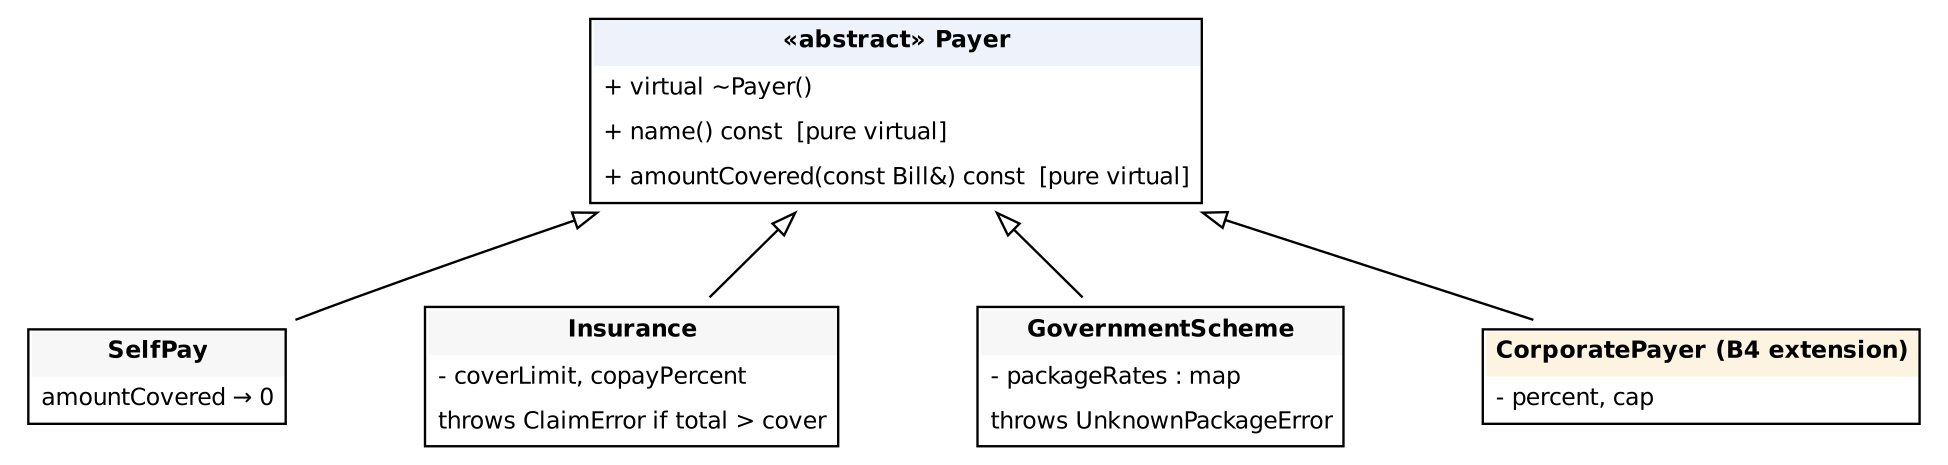
\includegraphics[width=0.95\linewidth]{uml_payer.png}
\caption{Payer hierarchy. The B4 extension adds CorporatePayer as a new subclass.}\label{fig:payer}
\end{figure}

\begin{lstlisting}[style=pseudo,caption={Pseudocode: Insurance.amountCovered}]
ALGORITHM InsuranceCovered(bill)
  INPUT : bill -- a Bill, coverLimit and copayPercent from the object
  OUTPUT: amount covered, or a rejected claim
  BEGIN
    t <- bill.total()
    IF t > coverLimit THEN
      THROW ClaimError("exceeds cover")
    END IF
    RETURN t * (1 - copayPercent / 100)
  END
\end{lstlisting}

\subsection*{A3.2 Extension without changing existing classes}
A new payer, \texttt{CorporatePayer} (a percentage cover with a per-claim cap), is added in a new file (\texttt{extension.hpp}). The class derives from \texttt{Payer} and overrides the two pure virtual functions. No existing class, header or function changes. Existing code that holds a \texttt{Payer\&} accepts the new payer at once.

\begin{lstlisting}[caption={extension.hpp: CorporatePayer (new payer, no existing class changed)}]
class CorporatePayer : public Payer {
    double percent, cap;
public:
    CorporatePayer(double pct, double capAmount) : percent(pct), cap(capAmount)
    {
        if (pct < 0 || pct > 100) throw BillingError("corporate percent out of range");
        requireNonNegative(capAmount, "corporate cap");
    }
    std::string name() const override { return "Corporate"; }
    double amountCovered(const Bill& b) const override
    {
        return std::min(b.total() * percent / 100.0, cap);
    }
};
\end{lstlisting}

\subsection*{Alternative concept: function pointers or std::function}
A payer could instead be a \texttt{std::function<double(const Bill\&)>} chosen at run time. Calling it is $O(1)$, the same as a virtual call. Space differs. A \texttt{std::function} stores a type-erased callable, usually 32 bytes in libstdc++, and a lambda that captures the cover limit stores the captured values inside that object. An abstract class stores the same data as named members. Named members are visible in a debugger and can be inspected and tested directly, and the captured-lambda form hides them. For this assignment, where payers carry several named parameters and must reject claims with specific error types, the class design is clearer. A function object is better when the rule is a single short expression.

%-------------------------------------------------------------
\section{Task A4 -- Design the Exception Strategy}
%-------------------------------------------------------------
\subsection*{A4.1 Errors and the exception hierarchy}
\begin{table}[H]
\centering
\small
\begin{tabular}{@{}p{4.2cm}p{4.6cm}p{5.8cm}@{}}
\toprule
\textbf{Error} & \textbf{Exception class} & \textbf{Raised by / handled by} \\
\midrule
Negative charge (consultation, tests, days, rate, surgery) & \texttt{NegativeChargeError} & Bill constructors (\texttt{requireNonNegative}); caught per claim \\
Claim above cover & \texttt{ClaimError} & \texttt{Insurance::amountCovered}; caught in \texttt{settleOne} as a rejection \\
Unknown package code & \texttt{UnknownPackageError} & \texttt{GovernmentScheme::amountCovered}; rejection recorded \\
Missing patient record & \texttt{MissingRecordError} & \texttt{Registry::find}; reported to the caller \\
Co-payment or corporate percent out of range & \texttt{BillingError} & Payer constructors; configuration error \\
Text where a number is expected & \texttt{std::invalid\_argument}, \texttt{std::out\_of\_range} & \texttt{std::stod} during input parsing \\
Memory allocation failure & \texttt{std::bad\_alloc} (standard) & Any allocation; reported at the top level \\
\bottomrule
\end{tabular}
\caption{Errors and their exception types. Every billing exception derives from \texttt{BillingError}, which derives from \texttt{std::runtime\_error} and therefore \texttt{std::exception}.}
\end{table}

\begin{figure}[H]
\centering
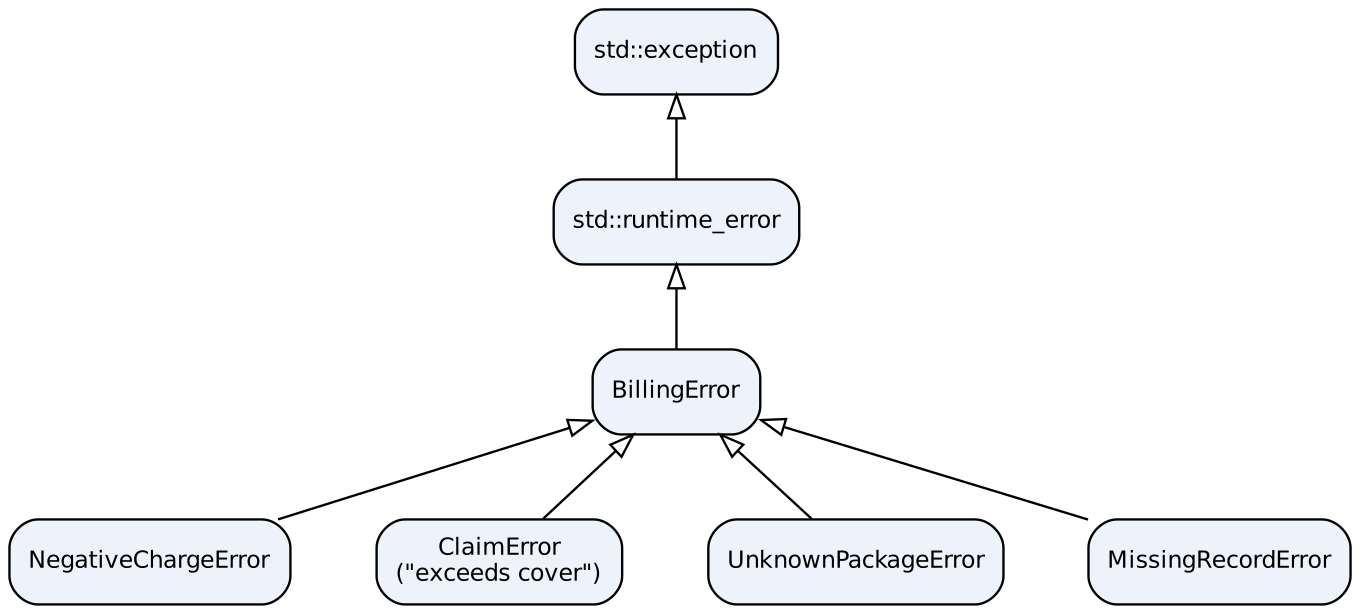
\includegraphics[width=0.75\linewidth]{uml_exceptions.png}
\caption{Exception class hierarchy.}\label{fig:exc}
\end{figure}

\subsection*{A4.2 Exception specifications}
Each function is classified as either may throw or must never throw. The must-never-throw functions are marked \texttt{noexcept}.

\begin{table}[H]
\centering
\small
\begin{tabular}{@{}p{5.8cm}p{2.2cm}p{6.6cm}@{}}
\toprule
\textbf{Function} & \textbf{Specification} & \textbf{Reason} \\
\midrule
\texttt{Bill::patientName() const} & \texttt{noexcept} & Returns a reference; cannot fail \\
\texttt{Bill::\~{}Bill()} and all destructors & implicitly \texttt{noexcept} & Must never throw (see below) \\
\texttt{Payer::amountCovered} & may throw & Rejects claims by throwing \\
\texttt{settleOne(...)} & may throw & Allocates the result string; \texttt{std::bad\_alloc} can escape \\
Constructors of bills and payers & may throw & Validate input and throw \texttt{NegativeChargeError} / \texttt{BillingError} \\
\bottomrule
\end{tabular}
\end{table}

\paragraph{Why destructors must not throw.} During stack unwinding, objects are destroyed while an exception is already active. If a destructor throws during this process, the program calls \texttt{std::terminate}, and the original exception is lost. Since C++11 destructors are implicitly \texttt{noexcept}, so an exception leaving a destructor terminates the program immediately. Destructors in this design only release memory or print a message.

\subsection*{Alternative concept: return codes}
Errors could instead be returned as an \texttt{enum Status} or with a \texttt{bool} and an output parameter. On the \textbf{normal path} this costs one comparison per call and no unwinding machinery, so it is $O(1)$ extra per call. On the \textbf{error path} each caller must test the status and pass it up, which costs an extra branch at every level, but no stack unwinding occurs. The measured cost of exceptions on the error path is about 1~microsecond per thrown error, against about 1~nanosecond for a return code (B3). The space cost is code size: every function that can fail carries a status parameter and a check at each call site, which grows with the number of call sites. The exception design keeps the normal code path clean and centralises error handling, at the price of a higher cost per error. Section~B3 shows that this price is paid only when errors occur.

%-------------------------------------------------------------
\section{Task A5 -- Design Recovery and Rethrowing}
%-------------------------------------------------------------
\subsection*{A5.1 Where each exception is caught}
\begin{itemize}[nosep]
\item \textbf{Leaf (raise).} Bill constructors and payers throw the specific error at the point the rule is broken, so the message names the cause.
\item \textbf{Middle (log and rethrow).} A function that can add context (for example the claim identifier) catches the exception, writes a log line, and rethrows it with \texttt{throw;} so the original object reaches the caller unchanged.
\item \textbf{Per claim (record and continue).} \texttt{settleOne} catches \texttt{BillingError}, records a rejection with its reason, and returns. The bill is kept in the batch result, so it is never lost.
\item \textbf{Top level (report to user).} \texttt{main} catches \texttt{std::exception} and \texttt{catch(...)}, reports the error, and continues with the next item.
\end{itemize}

\subsection*{A5.2 Stack unwinding and RAII}
When an exception leaves a block, the runtime destroys every automatic object that was constructed in that block, in reverse order of construction. This is \emph{stack unwinding}. A resource owned by an object is released by its destructor, so a \texttt{std::unique\_ptr}, \texttt{std::vector} or file stream never needs manual cleanup. Holding a resource in an object whose lifetime matches the resource's is called RAII (Resource Acquisition Is Initialisation). Because unwinding runs the destructors on every exit path, RAII removes leaks on error paths automatically.

\subsection*{Predict the output: program 2}
The program is given in the assignment (\texttt{Task02\_RAII\_Unwinding/predict\_a5.cpp}).

\begin{lstlisting}[caption={predict\_a5.cpp (as given)}]
#include <iostream>
#include <string>
struct Guard {
 std::string n;
 explicit Guard(const std::string& s) : n(s) {}
 ~Guard() { std::cout << '~' << n << ' '; }
};
void f()
{
 Guard g("f");
 throw 42;
}
int main()
{
 try {
 Guard m("main");
 f();
 std::cout << "not printed ";
 } catch (int x) {
 std::cout << "caught " << x;
 } catch (...) {
 std::cout << "other";
 }
 std::cout << '\n';
}
\end{lstlisting}

\textbf{Predicted output:} \texttt{\~{}f \~{}main caught 42} followed by a newline.

\textbf{Actual output} (\texttt{predict\_a5.out}):
\lstout{../Task02_RAII_Unwinding/predict_a5.out}{Actual output of predict\_a5}

\textbf{Explanation.} \texttt{throw 42} leaves \texttt{f()} immediately, so the statement after \texttt{f()} is never reached, which is why \texttt{not printed} never appears. Unwinding first destroys \texttt{g} in \texttt{f} (\texttt{\~{}f}), then destroys \texttt{m} in the \texttt{try} block of \texttt{main} (\texttt{\~{}main}). Only then does the matching handler run and print \texttt{caught 42}. The destructors run before the handler body, because the handler is entered only after the stack has been unwound to the \texttt{try} block. The predicted output matches the actual output.

\subsection*{Rethrow chain}
A two-level version (\texttt{rethrow\_chain.cpp}) shows the same effect with logging and \texttt{throw;}:

\lstout{../Task02_RAII_Unwinding/rethrow_chain.out}{Output of rethrow\_chain}

The lower-level guard is destroyed first, then the middle function logs and rethrows, its own guard is destroyed, and the top level reports the error. Every destructor ran once, and the error was logged once.

\subsection*{Alternative concept: delete in every catch block}
Without RAII, each function would release its own resources in every catch block and on every return path. The time cost is the same, because the same deallocations happen either way. The code size grows with the number of exit points. A function with $k$ resources and $m$ possible throw points needs up to $m$ cleanup sequences of $k$ deletes each, so there are $O(k \cdot m)$ places to get wrong. In the RAII design there are zero explicit cleanup sites. Each time a new error path is added, one new cleanup site must be written by hand, and forgetting one causes a leak that the compiler does not detect. Sanitizers detect leaks at run time only for paths that are tested.

%=============================================================
\part*{Part B -- Implementation and Experimental Investigation}
\addcontentsline{toc}{part}{Part B -- Implementation and Experimental Investigation}
%=============================================================

\section{Task B1 -- Implement and Validate the Polymorphic Billing}
\subsection*{B1.1 Validation with hand-calculated totals}
The library in \texttt{Task06\_Extension\_Final/billing.hpp} implements the hierarchy from A1 and the payers from A3. \texttt{main.cpp} tests one bill of each kind with each payer, and the expected values were calculated by hand before the test was written.

\begin{table}[H]
\centering
\small
\begin{tabular}{@{}llrrl@{}}
\toprule
\textbf{Bill} & \textbf{Payer} & \textbf{Hand calculation} & \textbf{Expected} & \textbf{Result} \\
\midrule
OP Ravi (500 + 1200) & SelfPay & 0 & 0 & PASS \\
OP Ravi & Insurance (cover 100000, copay 10\%) & $1700 \times 0.9$ & 1530 & PASS \\
OP Ravi & Government (OP rate 1000) & $\min(1000, 1700)$ & 1000 & PASS \\
OP Ravi & Corporate (50\%, cap 20000) & $1700 \times 0.5$ & 850 & PASS \\
IP Meena (3$\times$2500 + 40000) & Insurance & $47500 \times 0.9$ & 42750 & PASS \\
IP Meena & Government (IP rate 45000) & $\min(45000, 47500)$ & 45000 & PASS \\
IP Meena & Corporate & $\min(23750, 20000)$ & 20000 & PASS \\
DC Asha (package 30000) & Insurance & $30000 \times 0.9$ & 27000 & PASS \\
DC Asha & Government (DC rate 25000) & $\min(25000, 30000)$ & 25000 & PASS \\
DC Asha & Corporate & $\min(15000, 20000)$ & 15000 & PASS \\
\bottomrule
\end{tabular}
\caption{Verified totals for one bill of each kind and each payer (the full driver has 24 checks, all PASS).}
\end{table}

\lstout{../Task06_Extension_Final/billing_tests.out}{Full output of the test driver (B1.1, error paths, batch, B4.2 scope guards)}

\subsection*{B1.2 Comparison with the design}
Three changes were made to the A1 design during implementation.
\begin{enumerate}[nosep]
\item \texttt{type()} is pure virtual in the abstract base, so every bill must provide its own code. The assignment's TODO suggested a default return value of ``Bill''; the implementation keeps the default only in the completed Task03 program.
\item \texttt{print()} takes an \texttt{std::ostream\&} rather than writing to \texttt{std::cout}, so that tests can capture output.
\item Constructors validate their inputs and throw, which moves the negative-charge check from the calculation into the object's creation. An object with negative charges can never exist.
\end{enumerate}

\subsection*{B1.3 Proving run-time binding}
The completed program (\texttt{billing\_b1.cpp}) gives the expected output of \texttt{OP Ravi: 1700}, \texttt{IP Meena: 47500}, \texttt{Total 49200}.

\lstout{../Task03_Billing_CompleteCode/billing_b1.out}{Output of the completed B1 program (matches the expected output)}

When \texttt{virtual} is removed from \texttt{total()} in the \emph{pure} declaration, the code does not compile. Table~\ref{tab:b13} records the error. The pure virtual declaration \texttt{= 0} is only valid on a virtual function, and the derived \texttt{total()} then has nothing to override.

\lstout{../Task03_Billing_CompleteCode/compile_error_remove_virtual.txt}{Compiler error after removing virtual from the pure declaration of total()}

To observe the silent failure, the same program was modified so that \texttt{Bill} has a concrete non-virtual \texttt{total()} (\texttt{b13\_nonvirtual\_total.cpp}). This version compiles without warnings.

\lstout{../Task03_Billing_CompleteCode/b13_nonvirtual_total.out}{Output with non-virtual total(): every bill prints 0}

\begin{table}[H]
\centering
\small
\begin{tabular}{@{}lll@{}}
\toprule
\textbf{Version} & \textbf{Output} & \textbf{Why} \\
\midrule
virtual \texttt{total()} (correct) & 1700, 47500, total 49200 & Each bill's own \texttt{total()} is dispatched through its vtable \\
non-virtual \texttt{total()} & 0, 0, total 0 & \texttt{print()} calls the base function because the static type is \texttt{Bill} \\
\bottomrule
\end{tabular}
\caption{Effect of removing virtual from total(). Both programs compile. The second compiles without any warning and gives wrong totals.}\label{tab:b13}
\end{table}

\noindent The non-virtual version is more dangerous than the compile error, because it compiles and gives wrong numbers silently. A simpler demonstration (\texttt{nonvirtual\_total.cpp}) prints \texttt{0 500}: calling through a base pointer picks the base function, and calling through the derived type picks the derived function. This is static binding at work.

\subsection*{B1.4 Proving the virtual destructor}
The result of removing the virtual destructor under ASan was recorded in A2 above: \texttt{new-delete-type-mismatch}, with 32 bytes allocated and 8 bytes deallocated. The correct version with the virtual destructor (\texttt{predict\_a2\_asan.out}) runs with no sanitizer errors, and the output is \texttt{500 \~{}OPBill \~{}Bill}.

\subsection*{Alternative concept: templates (compile-time polymorphism)}
With templates, each bill type is handled in its own container and every call is resolved at compile time, so there is no vtable and no indirect call. The time per bill is the same order as a direct call, $O(1)$, and the space per bill is only the data, with no vptr. The loss is structural. A \texttt{std::vector<OutPatientBill>} and a \texttt{std::vector<InPatientBill>} cannot share one list, so a day's bills of mixed types need one loop per type and one container per type. A new type needs a new loop in every consumer. Virtual functions allow one heterogeneous list at the cost of one indirect call per bill. Section~B3 measures that cost.

%-------------------------------------------------------------
\section{Task B2 -- Engineer Error Conditions}
%-------------------------------------------------------------
\subsection*{Predict the output}
The program (\texttt{predict\_b2.cpp}) validates three amounts. The prediction was written from the rules before the run: \texttt{ok done} for 100; for $-5$, \texttt{std::invalid\_argument} is not caught by the \texttt{out\_of\_range} handler, so it escapes \texttt{process} and is printed by \texttt{main}; for $2 \times 10^6$, the \texttt{out\_of\_range} handler logs and rethrows.

\textbf{Predicted output:} \texttt{ok done caught negative [log too large] caught too large} followed by a newline.

\lstout{../Task04_ErrorHandling/predict_b2.out}{Actual output of predict\_b2}

\textbf{Explanation.} Only one exception is logged. The first exception (\texttt{invalid\_argument}) does not match the handler in \texttt{process}, so that handler never runs and nothing is logged. The second exception (\texttt{out\_of\_range}) matches, so it is logged and rethrown with \texttt{throw;}. The rethrow passes the same object up, where \texttt{main} catches it as \texttt{std::exception} and prints \texttt{caught too large}. The matching was based on the static type in each \texttt{catch}, so the handler order determined the outcome.

\subsection*{Complete the code: claim settlement}
\lstout{../Task04_ErrorHandling/claim_settle.cpp}{claim\_settle.cpp with TODO 1 and TODO 2 completed}

\lstout{../Task04_ErrorHandling/claim_settle.out}{Output: matches the expected output of the assignment}

The expected output is reproduced exactly. The \texttt{throw;} in \texttt{settle} rethrows the original \texttt{ClaimError}, which is why \texttt{main} catches it as \texttt{ClaimError} and prints \texttt{claim rejected}.

\subsection*{Replacing throw; with throw e;}
\lstout{../Task04_ErrorHandling/claim_settle_throw_e.out}{Output with throw e;}

The rethrown object is a copy made from the static type of \texttt{e}, which here is \texttt{std::runtime\_error}, not the dynamic type \texttt{ClaimError}. The copy is \emph{sliced}, so the derived part is lost. \texttt{main} then does not match the \texttt{ClaimError} handler and prints \texttt{error: exceeds cover}. Plain \texttt{throw;} rethrows the object with its dynamic type intact, so it is the correct choice in a handler.

\subsection*{Engineered error tests}
\lstout{../Task04_ErrorHandling/error_tests.out}{Output of the engineered error tests}

\noindent Each test reveals a specific property of the design:
\begin{itemize}[nosep]
\item \textbf{T1, T2} show that the typed hierarchy lets a handler select the exact failure (negative charge, claim above cover, unknown package).
\item \textbf{T3} shows that \texttt{std::stod} accepts a numeric prefix (\texttt{12abc} becomes 12), so the input layer must check the full string, which the exception type alone does not guarantee. \texttt{abc} raises \texttt{invalid\_argument}, and \texttt{1e400} raises \texttt{out\_of\_range}.
\item \textbf{T4} shows that the 2$^{60}$-element allocation fails with \texttt{std::bad\_array\_new\_length}, a subclass of \texttt{std::bad\_alloc}. The object \texttt{before-alloc} is still destroyed, which demonstrates RAII during the failure.
\item \textbf{T5} shows that an \texttt{int} exception (not derived from \texttt{std::exception}) is caught by \texttt{catch(...)}, and the batch continues. Every item's \texttt{Trace} destructor runs, including the one that threw.
\end{itemize}

\subsection*{Alternative concept: std::optional$<$double$>$}
Invalid claims can be rejected by returning \texttt{std::optional<double>}, which holds no value for a rejected claim. \texttt{optional\_vs\_exception.cpp} measures this for 1{,}000{,}000 claims.

\lstout{../Task04_ErrorHandling/optional_vs_exception.out}{Measured optional versus exception, 1,000,000 claims (-O2, median of 5)}

\noindent The optional version costs about 1.1~ms regardless of the invalid rate, whereas exceptions cost about 1~microsecond per invalid claim. At 50\% invalid, the exception design takes roughly 600~ms against about 1~ms. The extra space is 16 bytes per result for \texttt{optional<double>}, against 8 bytes for \texttt{double}. The optional design also cannot say \emph{why} a claim was rejected, which the exception types do. The trade-off is therefore between a faster rejection path with less information and a slower path with typed reasons.

%-------------------------------------------------------------
\section{Task B3 -- Virtual Functions vs Switch vs Exceptions: The Cost}
%-------------------------------------------------------------
\subsection*{B3.1 Correctness on small data}
\lstout{../Task05_Performance/bench_O2.out}{Full benchmark output (first part shows B3.1 correctness)}
The virtual, switch and \texttt{std::variant} designs gave the same total on 10 bills (246095.0), so the three versions agree.

\subsection*{B3.2 Increasing the data size (-O2)}
Table~\ref{tab:b32} gives the median of 5 runs. The full output is above. A second, independent run gave the same ordering at every size.

\begin{table}[H]
\centering
\small
\begin{tabular}{@{}rlrrrr@{}}
\toprule
\textbf{$n$} & \textbf{Design} & \textbf{Run 1 (ms)} & \textbf{Run 1 (ns/bill)} & \textbf{Run 2 (ms)} & \textbf{Run 2 (ns/bill)} \\
\midrule
1{,}000 & virtual & 0.002 & 2.48 & 0.002 & 2.40 \\
1{,}000 & switch & 0.001 & 0.64 & 0.001 & 0.63 \\
1{,}000 & variant & 0.001 & 0.64 & 0.001 & 0.61 \\
\midrule
1{,}000{,}000 & virtual & 4.055 & 4.06 & 3.778 & 3.78 \\
1{,}000{,}000 & switch & 1.748 & 1.75 & 1.718 & 1.72 \\
1{,}000{,}000 & variant & 2.249 & 2.25 & 2.284 & 2.28 \\
\midrule
10{,}000{,}000 & virtual & 47.363 & 4.74 & 39.114 & 3.91 \\
10{,}000{,}000 & switch & 23.279 & 2.33 & 21.688 & 2.17 \\
10{,}000{,}000 & variant & 26.995 & 2.70 & 26.349 & 2.63 \\
\bottomrule
\end{tabular}
\caption{Time to total $n$ bills (-O2). The 1{,}000-bill timings are at the limit of the clock's resolution and are included for completeness.}\label{tab:b32}
\end{table}

\noindent All three designs are $O(n)$. The per-bill cost is roughly constant with $n$. The virtual design is about 1.8 to 2 times slower than the switch, because each call is an indirect jump. In this data the two kinds alternate, which may be easy for the branch predictor; this was not tested. Data with a random kind order could change the gap, and it is a question for further measurement. The \texttt{std::variant} design sits between the two. The space per element measured with \texttt{sizeof} was 24 bytes for the switch record, 32 bytes for \texttt{VarBill}, and 24 bytes for \texttt{VOP} plus 8 bytes for the \texttt{unique\_ptr} and a heap allocation header for the virtual version.

\subsection*{B3.3 Cost of exceptions}
Each validation was repeated for 1{,}000{,}000 bills with 0\%, 1\% and 50\% invalid.

\begin{table}[H]
\centering
\small
\begin{tabular}{@{}rlrr@{}}
\toprule
\textbf{Invalid \%} & \textbf{Design} & \textbf{Time (ms)} & \textbf{Rejected} \\
\midrule
0 & return code & 1.096 & 0 \\
0 & exception & 0.943 & 0 \\
1 & return code & 1.128 & 10{,}000 \\
1 & exception & 10.871 & 10{,}000 \\
50 & return code & 1.112 & 500{,}000 \\
50 & exception & 490.592 & 500{,}000 \\
\bottomrule
\end{tabular}
\caption{Validation of 1{,}000{,}000 bills (-O2, median of 5).}\label{tab:b33}
\end{table}

\noindent With no errors, both designs cost about 1~ms. Each thrown exception costs about 1~microsecond: $(10.871 - 0.943) / 10\,000 \approx 0.99\,\mu\text{s}$ at 1\%, and $(490.592 - 0.943) / 500\,000 \approx 0.98\,\mu\text{s}$ at 50\%. The cost is paid per error, not per bill.

\subsection*{B3.4 Engineering trade-off}
The results separate two situations.
\begin{itemize}[nosep]
\item \textbf{Virtual dispatch} costs about 2 to 4~ns per bill in this measurement. Its price is paid on every bill, but it is small. The switch is faster but must be edited for each new type, so it suits a closed, stable set of types. Virtual functions suit an open set of types that grows over time.
\item \textbf{Exceptions} cost nothing on the normal path, but about 1~$\mu$s per error. They suit rare, serious failures such as an invalid claim that must be reported with a reason and must not be ignored. They are costly when errors are frequent, as at 50\% invalid, where the cost is about 500 times the return-code design. Return codes or \texttt{std::optional} suit routine validation where rejection is common.
\end{itemize}

\subsection*{Alternative concept: std::variant with std::visit}
\texttt{std::variant<VarOP, VarIP>} stores one alternative in place with a tag. Its time for 10{,}000{,}000 bills was 26.3--27.0~ms, between the switch (21.7--23.3~ms) and the virtual version (39.1--47.4~ms). Its space is 32 bytes per element, the size of the largest alternative plus the tag, with no heap allocation per element. The variant has the same extension cost as a switch, since adding an alternative changes the variant type and every \texttt{visit}. The compiler checks that every alternative is handled, which the switch does not do unless a warning is enabled.

%-------------------------------------------------------------
\section{Task B4 -- Final Engineering Decision}
%-------------------------------------------------------------
\subsection*{B4.1 Practical extension}
A new bill type (\texttt{DayCareBill}, package price) and a new payer (\texttt{CorporatePayer}) were added in \texttt{extension.hpp}. Neither \texttt{billing.hpp} nor any existing class was modified after it was first written. The full test driver includes the earlier checks and the extension checks, and all 24 PASS.

\subsection*{B4.2 Resource safety}
The test driver was compiled with \texttt{-fsanitize=address,undefined} and run. Exceptions were thrown and caught in several places, including a rejected claim, a negative charge, and a missing record. The sanitizer produced no errors and LeakSanitizer reported no leaks.

\lstout{../Task06_Extension_Final/billing_tests_asan.out}{Tail of the ASan and UBSan run: exception paths caught, scope guards destroyed, no sanitizer report}

\noindent The error tests were also run with ASan. The allocation test requires \texttt{allocator\_may\_return\_null=1} under ASan, which allows the allocation to return \texttt{nullptr}, not abort, so that the \texttt{std::bad\_alloc} path is exercised.

\lstout{../Task04_ErrorHandling/error_tests_asan.out}{Output of error\_tests under ASan (allocator\_may\_return\_null=1)}

\subsection*{B4.3 Production decision}
\textbf{Decision:} adopt the polymorphic design with exceptions for the billing system.

\noindent \textbf{Justification.} The workload is 200{,}000 bills per day. Using the measured costs:
\begin{itemize}[nosep]
\item Dispatch: about 4~ns per bill, so $200{,}000 \times 4\,\text{ns} \approx 0.8$~ms per day. Dispatch is not a bottleneck.
\item Errors: even if every claim were rejected, the exception cost is about $200{,}000 \times 1\,\mu\text{s} = 0.2$~s per day, and with a 50\% rejection rate about 0.1~s. The real time is spent in database and network access, which is many orders of magnitude larger.
\item Extension: a new bill type or payer requires one new class and one new file, with no edits to tested code. The effort of extension is the largest cost of the system, and this design minimises it.
\end{itemize}

\noindent \textbf{Condition.} If a future bulk screening pipeline rejects a large share of records and must process them at memory speed, the screening stage should use \texttt{std::optional} or return codes. Exceptions remain at the claim boundary where a rejection must carry a reason.

\subsection*{Alternative concept: configuration-driven plug-ins}
If new bill types and payers were loaded from configuration files describing rates and rules, the time per bill would be the cost of interpreting the rule rather than one virtual call. For a rule with $r$ terms this is $O(r)$ per bill, with a larger constant than dispatch. The space needed is the parsed rule table, which is small compared with the bill data. The effort of extension falls, since a new rate needs no compilation and no release. The risk rises. The type system no longer checks that a rule is well formed, so an error in a configuration file can silently produce wrong totals on all 200{,}000 daily bills. This alternative was not measured. The estimate is that the rule interpretation cost is a small multiple of a virtual call, but the risk of silent error is the deciding factor for a billing system, and the compiled design is preferred.

%=============================================================
\section{Conclusion}
%=============================================================
The programs show the progression requested by the assignment. Abstract base classes with virtual functions let new bill and payer types be added without changing working code, and the virtual destructor and vtable behaviour were verified with the sanitizer. Exceptions carry typed reasons for each rejected claim and are caught at the correct level, with RAII releasing resources on every path. The measurements show that virtual dispatch costs a few nanoseconds per bill and that exceptions cost about one microsecond per error, which is acceptable at 200{,}000 bills per day. The design answers the key question of the assignment: new kinds of bills and payers can be added safely, and the program stays correct and leak-free when things go wrong.

%=============================================================
\appendix
\section{Key Source Listing: Extension Header}
%=============================================================
The full sources, outputs and sanitizer logs are in the repository. The main extension file is reproduced here.
\lstinputlisting[caption={extension.hpp}]{src/extension.hpp}

\end{document}
